
\section{Description of the IMMD System}

The IMMD system is composed of 4 identical modules which can be connected in series or parallel on the DC link. A 2 kW 3-phase GaN based motor drive inverter printed circuit board (PCB) and a control PCB are designed for the system. Total system output power is 8 kW and the module DC link voltage is 270 V.

\subsection{GaN based motor drive module}

The photograph of the 3-phase inverter module of the IMMD system is shown in Fig. \ref{fig:invertermodule} excluding the heat sink. The module consists of half-bridge legs with GaN FETs having 650 V and 30 A ratings. Each leg has a 5 $\mu F$ metal film capacitor, isolated gate driver dedicated to each GaN and a phase current measurement circuit. The DC link capacitor size is determined according to required capacitance which is calculated based on voltage ripple and required current rating \cite{Ugur2017}, by also taking the effect of interleaving into account. It is aimed to minimize the gate loop and power loop inductances keeping DC link film and ceramic capacitors as close as possible.

\begin{figure}[tb]
\begin{minipage}[b]{.4\linewidth}
\centering
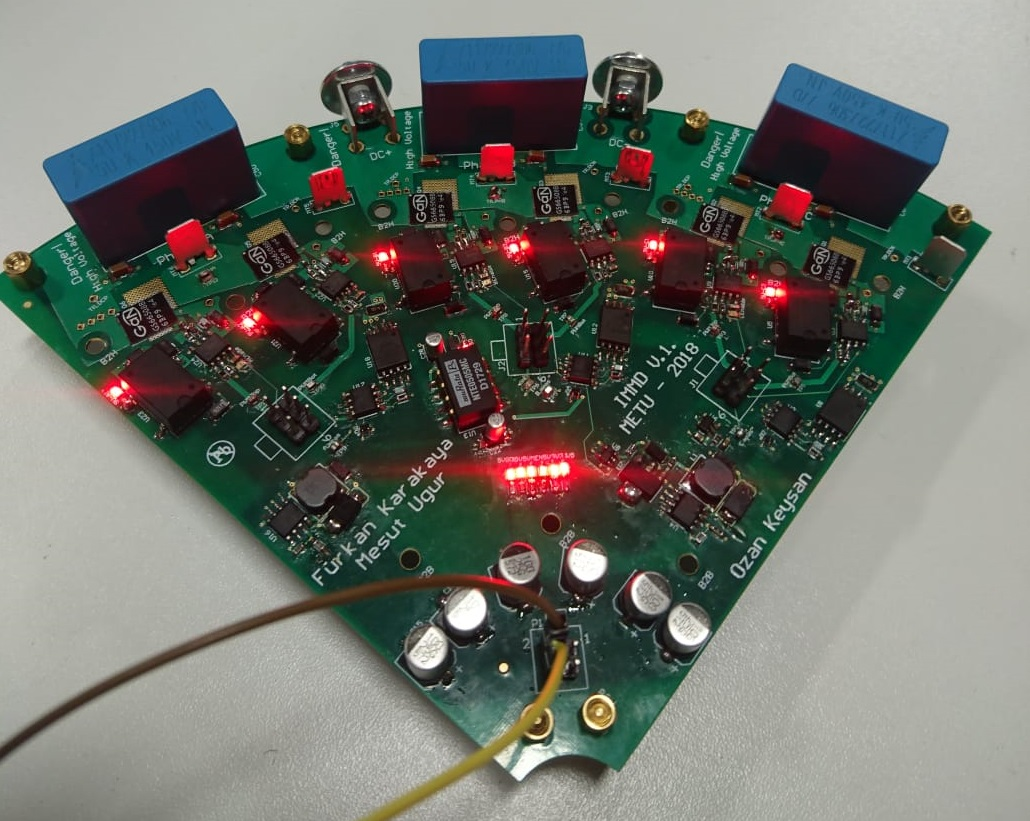
\includegraphics[width=6cm]{figures/invertermodule.jpg}
\caption{GaN based 3-phase inverter module}
\label{fig:invertermodule}
\end{minipage}%
\begin{minipage}[b]{.6\linewidth}
\centering
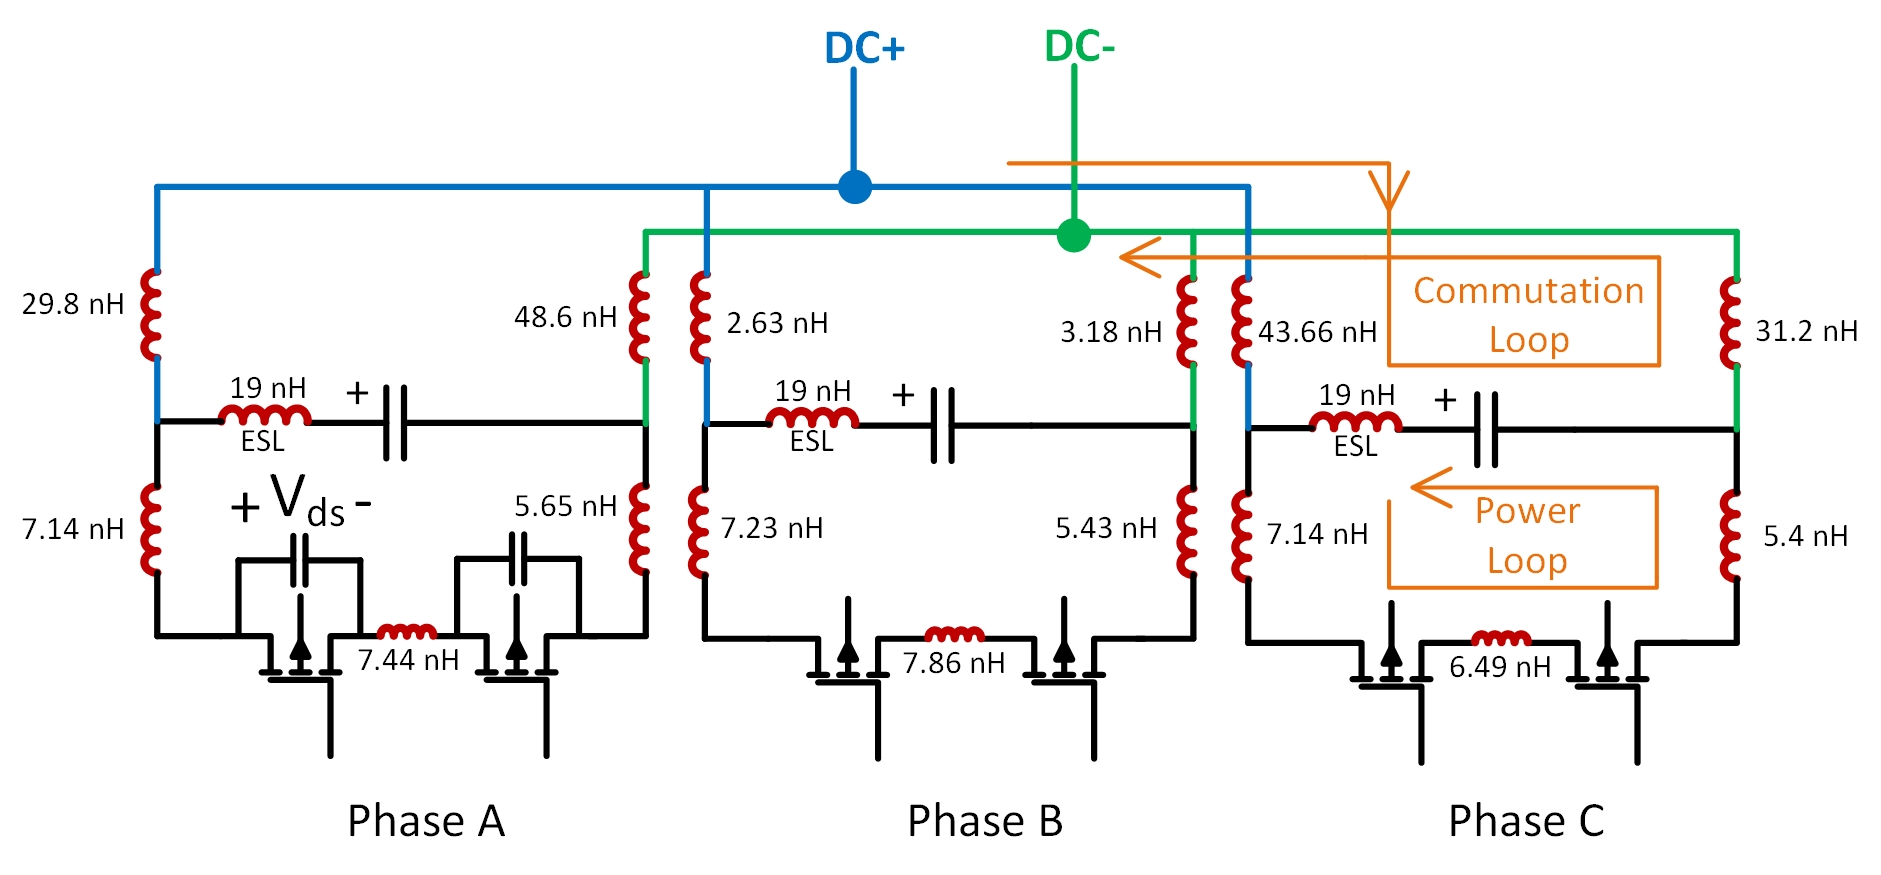
\includegraphics[width=10cm]{figures/SingleModuleInductanceMap.jpg}
\caption{Parasitic Inductance Map of a Single Module}
\label{fig:SingleModuleInductanceMap}
\end{minipage}
\end{figure}

\subsection{Parasitic Inductances}

For the inverter circuit given in Fig. \ref{fig:invertermodule}, the power loop and commutation loop inductances are identified using ANSYS/Q3D tool and given in Fig. \ref{fig:SingleModuleInductanceMap}. The power loop is effective when a commutation occurs between transistors on a single half-bridge while the commutation loop is effective whenever a current commutes from one phase to another.

\begin{figure}[tb]
\begin{minipage}[b]{0.6\linewidth}
\centering
\subfloat[\label{fig:SeriesModules}Series]{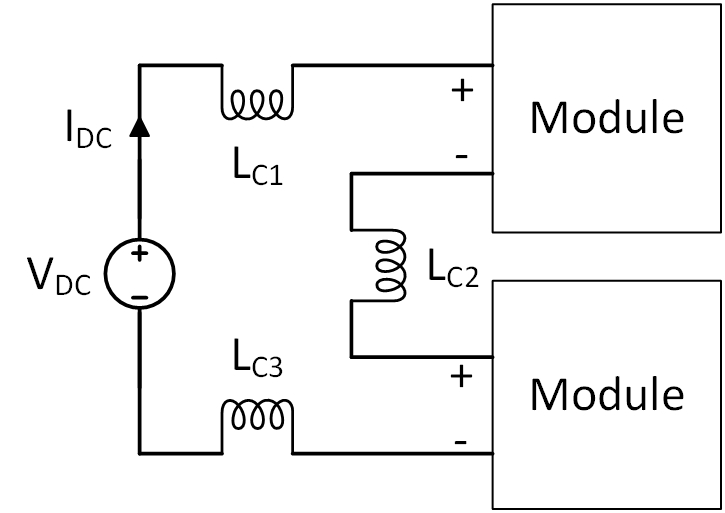
\includegraphics[width=4.5cm]{figures/SeriesModules.jpg}}\quad
\subfloat[\label{fig:ParallelModules}Parallel]{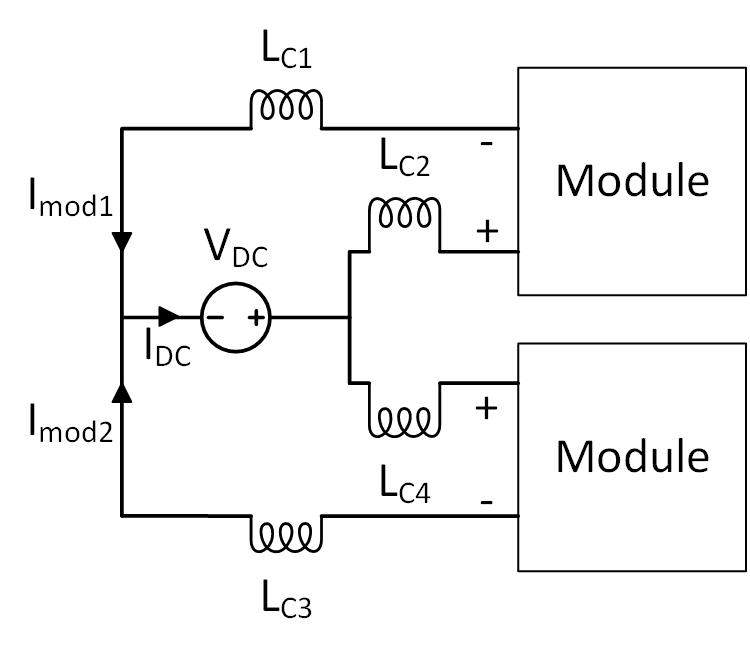
\includegraphics[width=4.5cm]{figures/ParallelModules.jpg}}
\caption{\label{fig:ModuleConnections}Series and Parallel Connected Modules Configurations}
\end{minipage}
\begin{minipage}[b]{0.4\linewidth}
\centering
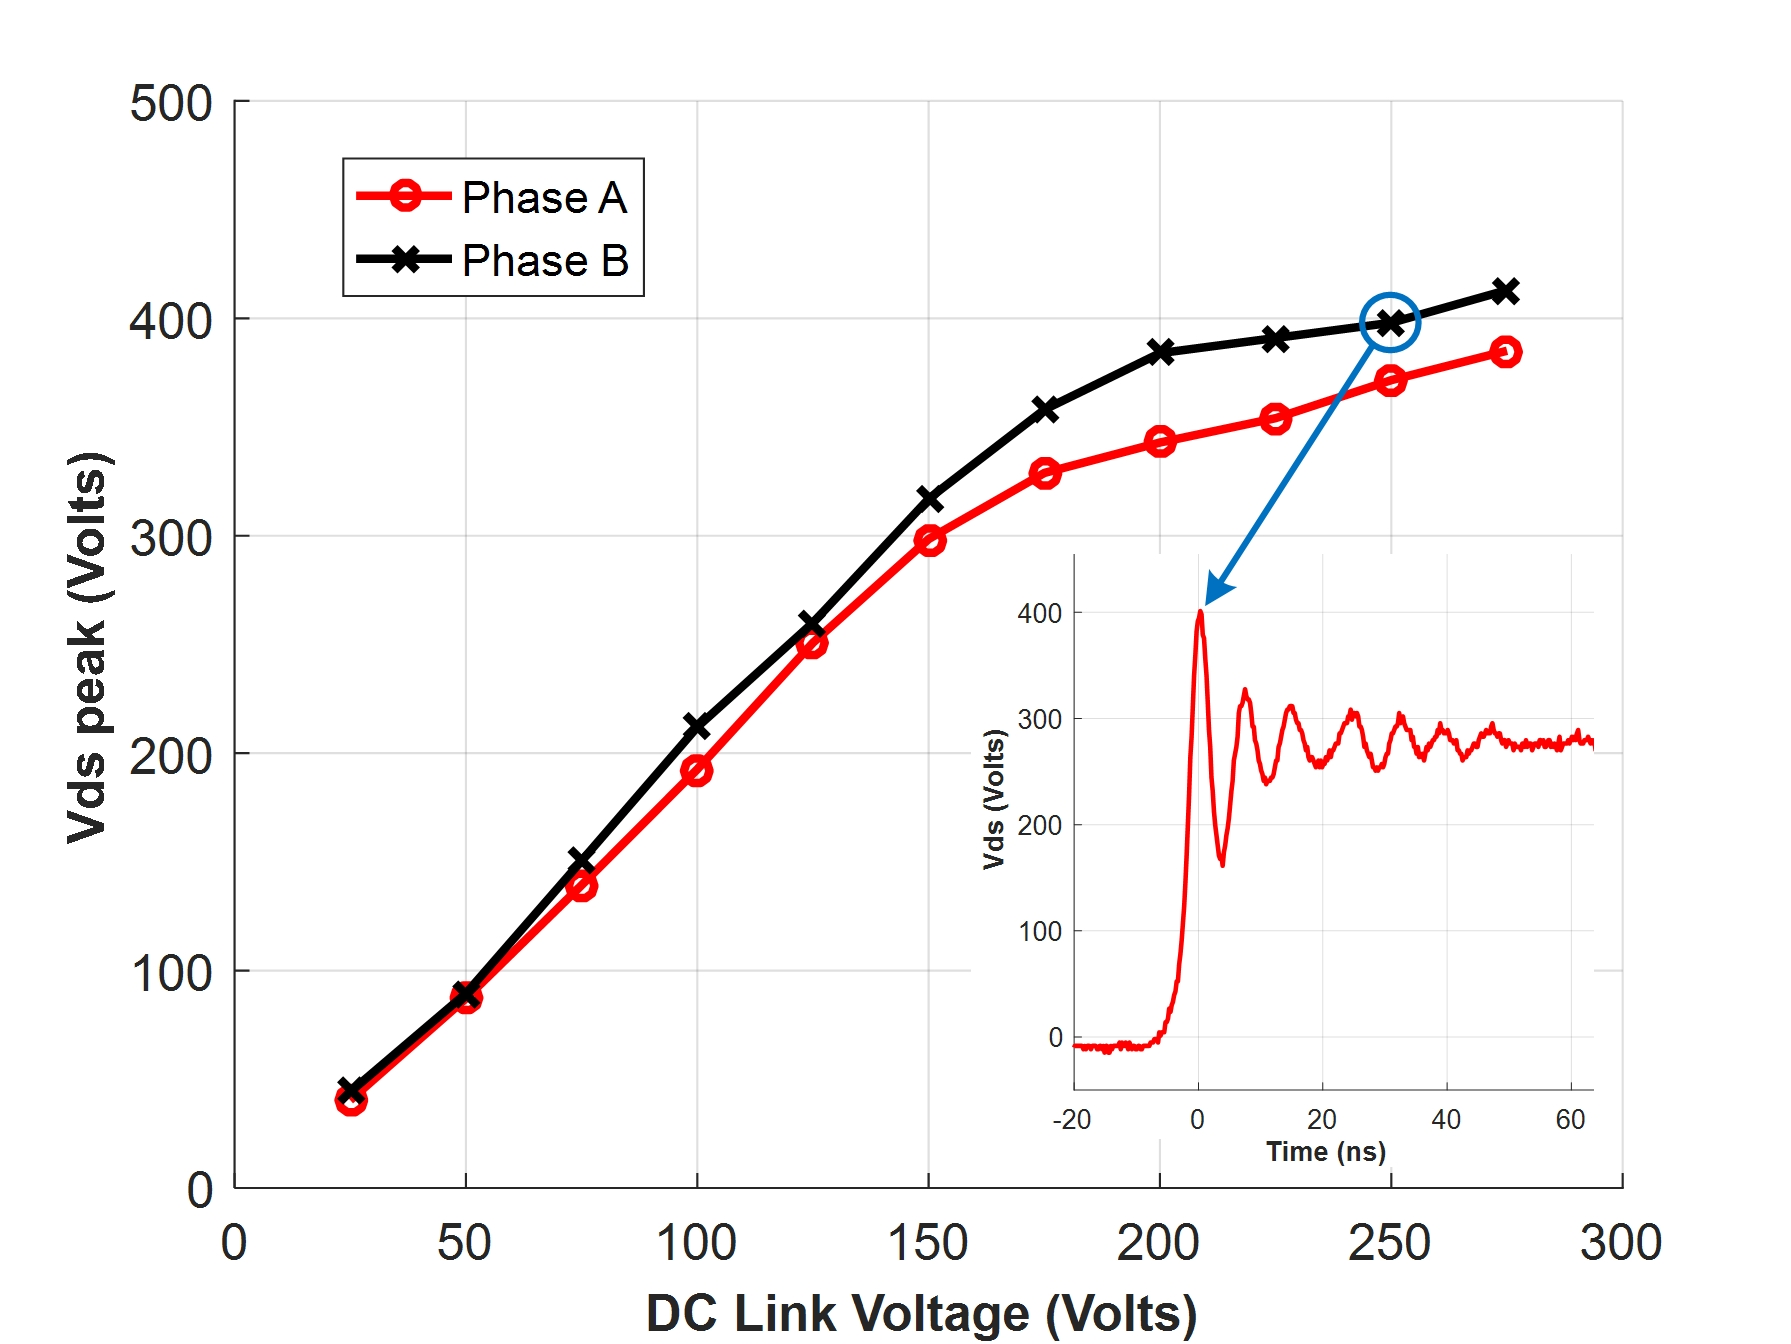
\includegraphics[width=7cm]{figures/experimentalvds2.jpg}
\caption{Experimental voltage overshoot results}
\label{fig:experimentalvds2}
\end{minipage}
\end{figure}

\subsection{Series and Parallel Connection}

As shown in Fig. \ref{fig:ModuleConnections}, two modules can be connected in series or parallel. The inductances given in Fig. \ref{fig:SeriesModules}, $L_{C1} \And L_{C3}$, are total equivalent inductances of connectors and module to supply terminal connections and $L_{C2}$ represents the total inductance of connectors and module to module connection. Similar inductances are also present in parallel connection.
